\documentclass{article}
\usepackage[paperwidth=19.5cm,paperheight=10.5cm,margin=0cm,noheadfoot]{geometry}
\usepackage{amsmath,amssymb}
\usepackage{tikz}
\usetikzlibrary{arrows.meta,positioning,calc,backgrounds,}
\usepackage{xcolor}
\usepackage[T1]{fontenc}
\usepackage{lmodern}
\usepackage{tgheros}
\usepackage{sansmath}
\renewcommand{\familydefault}{\sfdefault}
\sansmath
\pagestyle{empty}
\setlength{\parindent}{0pt}

% === Colors (consistent with Fig 4 KL palette) ===
\definecolor{deepblue}{HTML}{1A5276}
\definecolor{midblue}{HTML}{2980B9}
\definecolor{lightblue}{HTML}{D4E6F1}
\definecolor{bgblue}{HTML}{EBF5FB}

\definecolor{deepgreen}{HTML}{1E6B3A}
\definecolor{midgreen}{HTML}{27AE60}
\definecolor{lightgreen}{HTML}{A9DFBF}
\definecolor{bggreen}{HTML}{EAFAF1}

\definecolor{coralpink}{HTML}{E74C3C}
\definecolor{lightcoral}{HTML}{FADBD8}
\definecolor{deepgray}{HTML}{2C3E50}
\definecolor{midgray}{HTML}{7F8C8D}
\definecolor{panelbg}{HTML}{FAFCFE}

\begin{document}
\vspace*{0pt}\noindent
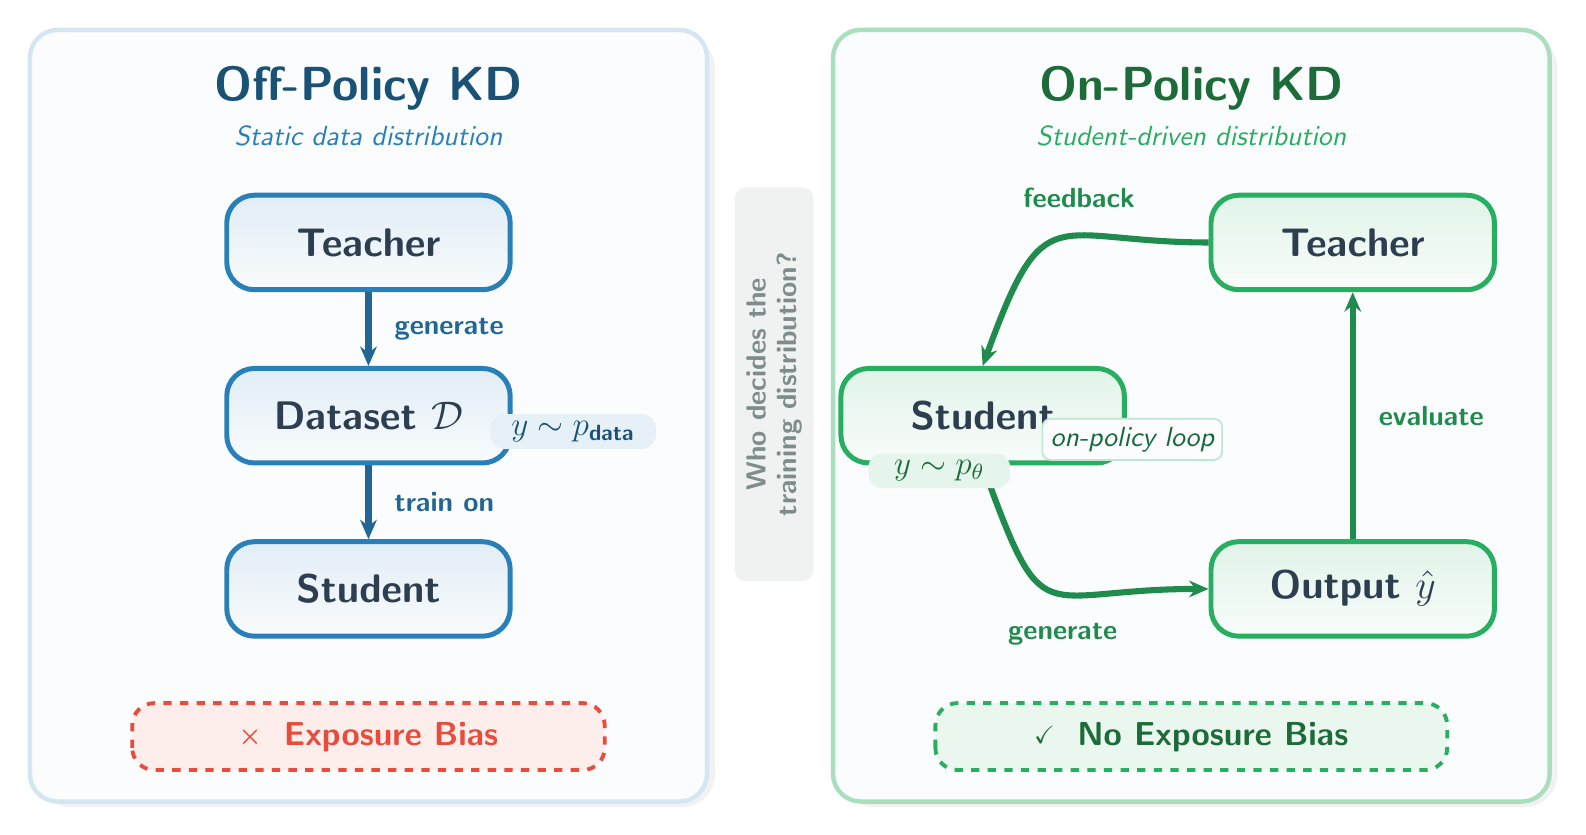
\begin{tikzpicture}[
    >=Stealth,
    bigbox/.style={
      draw=#1, line width=1.8pt, rounded corners=10pt,
      top color=#1!14, bottom color=#1!3,
      font=\Large\bfseries, minimum width=3.6cm, minimum height=1.2cm,
      text centered, inner sep=8pt, text=deepgray,
    },
    arr/.style={-{Stealth[length=7pt,width=6pt]}, line width=2.2pt, #1},
    lbl/.style={font=\normalsize\bfseries, #1},
  ]

  % =================== LEFT CARD: Off-Policy KD ===================
  % Shadow
  \fill[black, opacity=0.05, rounded corners=12pt] (0.1, -1.27) rectangle (8.7, 8.53);
  % Background
  \fill[panelbg, rounded corners=10pt] (0, -1.2) rectangle (8.6, 8.6);
  \draw[lightblue, line width=1.6pt, rounded corners=10pt] (0, -1.2) rectangle (8.6, 8.6);

  % Title
  \node[font=\LARGE\bfseries, deepblue] at (4.3, 7.85) {Off-Policy KD};
  \node[font=\normalsize\itshape, midblue] at (4.3, 7.25) {Static data distribution};

  % Boxes — linear flow
  \node[bigbox=midblue] (T1) at (4.3, 5.9) {Teacher};
  \node[bigbox=midblue] (D1) at (4.3, 3.7) {Dataset $\mathcal{D}$};
  \node[bigbox=midblue] (S1) at (4.3, 1.5) {Student};

  % Arrows
  \draw[arr=midblue!80!black] (T1) -- (D1)
    node[midway, right, lbl=midblue!80!black, xshift=5pt] {generate};
  \draw[arr=midblue!80!black] (D1) -- (S1)
    node[midway, right, lbl=midblue!80!black, xshift=5pt] {train on};

  % Distribution badge
  \fill[midblue!12, rounded corners=5pt] (5.85, 3.28) rectangle (7.95, 3.72);
  \node[font=\large\bfseries, deepblue] at (6.9, 3.5) {$y \sim p_{\text{data}}$};

  % Warning badge — Exposure Bias
  \fill[coralpink!10, rounded corners=8pt] (1.3, -0.8) rectangle (7.3, 0.05);
  \draw[coralpink, line width=1.4pt, rounded corners=8pt, dashed] (1.3, -0.8) rectangle (7.3, 0.05);
  \node[font=\large\bfseries, coralpink] at (4.3, -0.38) {\raisebox{0.5pt}{\small$\boldsymbol{\times}$}\; Exposure Bias};

  % =================== DIVIDER ===================
  \fill[midgray!12, rounded corners=4pt] (8.95, 1.6) rectangle (9.95, 6.6);
  \node[font=\normalsize\bfseries, midgray, rotate=90, text width=4.5cm, align=center] at (9.45, 4.1)
    {Who decides the\\[-1pt]training distribution?};

  % =================== RIGHT CARD: On-Policy KD ===================
  % Shadow
  \fill[black, opacity=0.05, rounded corners=12pt] (10.3, -1.27) rectangle (19.4, 8.53);
  % Background
  \fill[panelbg, rounded corners=10pt] (10.2, -1.2) rectangle (19.3, 8.6);
  \draw[lightgreen, line width=1.6pt, rounded corners=10pt] (10.2, -1.2) rectangle (19.3, 8.6);

  % Title
  \node[font=\LARGE\bfseries, deepgreen] at (14.75, 7.85) {On-Policy KD};
  \node[font=\normalsize\itshape, midgreen] at (14.75, 7.25) {Student-driven distribution};

  % Boxes — triangle layout
  \node[bigbox=midgreen] (S2) at (12.1, 3.7) {Student};
  \node[bigbox=midgreen] (O2) at (16.8, 1.5) {Output $\hat{y}$};
  \node[bigbox=midgreen] (T2) at (16.8, 5.9) {Teacher};

  % Cycle arrows — on-policy loop
  \draw[arr=midgreen!80!black] (S2.south) .. controls ++(0.8,-2.2) and ++(-2.2,0) .. (O2.west)
    node[pos=0.55, below, lbl=midgreen!80!black, yshift=-6pt] {generate};
  \draw[arr=midgreen!80!black] (O2.north) -- (T2.south)
    node[midway, right, lbl=midgreen!80!black, xshift=5pt] {evaluate};
  \draw[arr=midgreen!80!black] (T2.west) .. controls ++(-2.0,0) and ++(0.8,2.2) .. (S2.north)
    node[pos=0.4, above, lbl=midgreen!80!black, yshift=6pt] {feedback};

  % Loop indicator — center of triangle
  \node[font=\normalsize\itshape, midgreen!60!black, fill=panelbg, inner sep=3pt, rounded corners=3pt,
        draw=midgreen!30, line width=0.6pt] at (14.0, 3.4) {on-policy loop};

  % Distribution badge
  \fill[midgreen!12, rounded corners=5pt] (10.65, 2.78) rectangle (12.45, 3.22);
  \node[font=\large\bfseries, deepgreen] at (11.55, 3.0) {$y \sim p_\theta$};

  % Success badge — No Exposure Bias
  \fill[midgreen!10, rounded corners=8pt] (11.5, -0.8) rectangle (18.0, 0.05);
  \draw[midgreen, line width=1.4pt, rounded corners=8pt, dashed] (11.5, -0.8) rectangle (18.0, 0.05);
  \node[font=\large\bfseries, deepgreen] at (14.75, -0.38) {\raisebox{0.5pt}{\small$\boldsymbol{\checkmark}$}\; No Exposure Bias};

\end{tikzpicture}
\end{document}
